\chapter{Introduction}
Despite the fact that station safety is a crucial component of the overall structure of railway networks, accidents at stations continue to happen. It's essential to learn from these mistakes and advance traditional practices by analysing incidents and enhancing safety systems using cutting-edge technology, such as machine learning (ML) \cite{alawad_learning_2020}. Digital technologies can suggest better safety practices by mining complex patterns and hidden relationships from the existing data. The insights generated through sophisticated analytical tools will be helpful in the decision-making process to mitigate safety risks at stations. The decision tree method is particularly useful in this scenario as it explicitly represents decisions and decision making. This model is preferable because its structured rules are simple to follow and understand. 

Here, we explore the employment of decision tree (DT) method in safety classification and analysis of accidents at railway stations to predict the traits of passengers affected by the accidents.

\section{Background}
The machine learning technique has proven to be an effective tool in various fields. The application of ML has become more attractive due to the progressive refinement of its models, its reduced cost, and the improvement of employees' skills and lifestyles \cite{EDIEKMANN199275}. The decision tree method is a commonly used data mining method for establishing classification systems based on multiple covariates or for developing prediction algorithms for a target variable. This method classifies a population into branch-like segments that construct an inverted tree with a root node, internal nodes, and leaf nodes \cite{song_decision_2015}.\\ 
Here DT method is used to analyse the history of accidents in UK stations collected from RSSB \footnote{The Rail Safety and Standards Board is the independent safety standards and research body for Great Britain’s rail network. Website: https://www.rssb.co.uk/en} reports. Furthermore, a framework for railway station safety benefits based on both internal and external safety data and real-time data to enable the construction of smart stations in the future is proposed. 

\section{Related works}
Researchers from all over the world are looking into how cutting-edge technology like ML and DL might be used to improve safety at railway systems. Real time as well as historical data can be analysed to propose safety improvements by learning patterns from the data. 

Gilbert in his work, explores the possibility of implementing automatic track inspection system by employing deep learning techniques on data collected by track inspection vehicle.  A method for detecting obstacles by comparing input and reference train frontal view camera images is developed \cite{gilbert_2017}. 

Video cameras and sensors are some examples for sources of real time data, which can be used for real time analysis and prediction. Training ML and DL models on the data will be helpful to create powerful systems that can improve safety at railway stations. Traditional track inspection by laser ultrasonic imaging test takes a long time and cannot achieve large area scanning of rail. Combining the laser-ultrasonic technology and a hybrid intelligent method (using DL) may improve the speed of classification and evaluation of rolling contact fatigue (RCF) defect in different depths \cite{jiang_fast_2019}. Deep learning methods like CNN can be applied on images collected by inspection vehicle for automatic visual inspection and object detection\cite{han_deep_2020}. 

Another important source of data is historical records collected by authorities. The database of accident reports of past incidents can be used to train ML models for intelligent ranking of accidents. This model will then rank future incidents before analysed by human operators \cite{bikov_railway_2017}. This model helps to classify accidents based on severity and hence ease the manual work. 

Another notable work is by Heidarysafa \cite{heidarysafa_analysis_2018} in which accidents are classified based on narrative text on accident reports. Deep learning and text mining techniques are used for this purpose.

Examples of studies utilising advanced methods in railway applications are summarized in Figure \ref{fig:related_works}

\begin{figure}
    \centering
    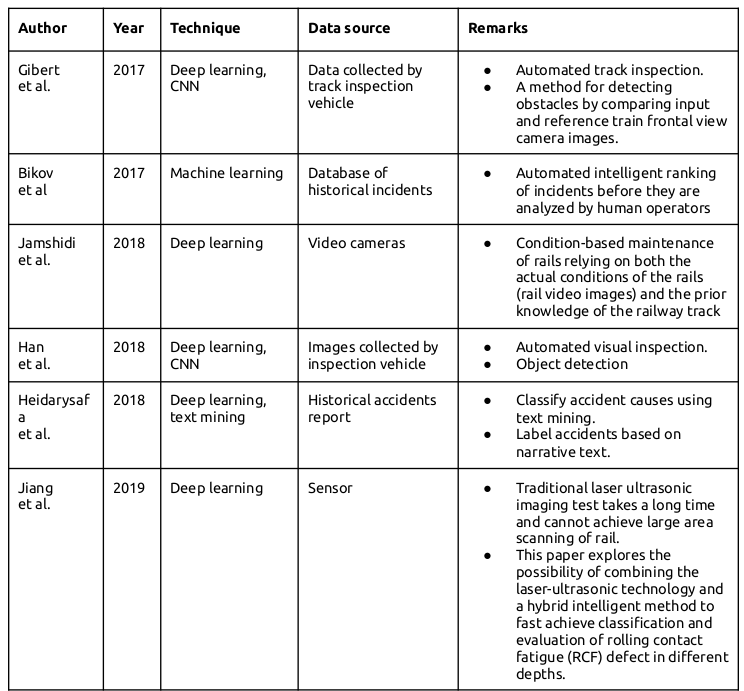
\includegraphics[scale=.4]{chapters/images/related_works.png}
    \caption{Studies related to utilising advanced digital technologies in railway applications.}
    \label{fig:related_works}
\end{figure}

\section{Methodology}
Conventionally, a data science process has the following stages;
\begin{enumerate}
    \item Data preparation
    \item Modelling
    \item Model evaluation
    \item Deployment 
\end{enumerate}
This is shown in Figure \ref{fig:metho}. We will see each stage in detail. 

\begin{figure}
    \centering
    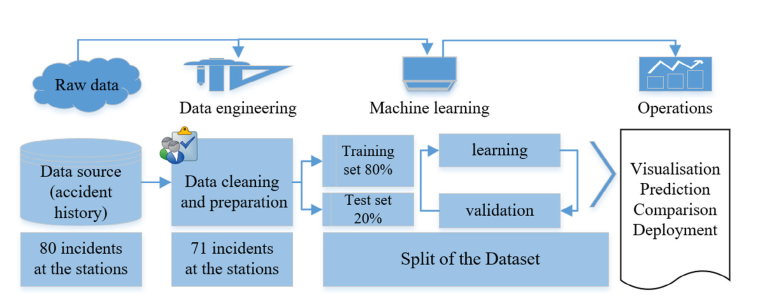
\includegraphics[scale=0.3]{chapters/images/methodology.png}
    \caption{Overview of all processes involved in a data science project}
    \label{fig:metho}
\end{figure}

\subsection{Data preparation}
It is one of the most time consuming activities in the entire process. This involves mainly two activities. 
\begin{enumerate}
    \item Data collection 
    \item Data cleaning
\end{enumerate}
Data collection is the process of collecting data from various sources. Finding reliable source is important. Data collected may be in structured, unstructured or semi-structured form. Real world data is often complex and hence may need some processing before it can be used for analysis and modelling. Accuracy of the analysis and modelling depends on the quality of data. Therefore this has to be done carefully. 

\subsection{Modelling}
A model is the abstract representation of the data and the relationships in a given data set \cite{kotu_data_2019}.There are several modelling algorithms available to work with different types of data. Choice of a learning algorithm depends on type of the data and our objectives. Here, we apply decision tree method for analysis and prediction. A portion of data set is used to train the model. This is called training data set. Another portion of data is used to evaluate the model. Subset of data used for testing is called testing data set. Typically, we choose 80\% of the data for training and 20\% for testing. 

\subsection{Model evaluation}
Before proceeding to deploy the system, accuracy and reliability of model must be tested and verified. The training and evaluation processes are iterative in nature. Different algorithms are tried and performances are evaluated, and corrections are made if necessary. One way to calculate the accuracy of the model is by building confusion matrix. In the field of machine learning and specifically the problem of statistical classification, a confusion matrix, also known as an error matrix,\cite{stehman_selecting_1997} is a specific table layout that allows visualization of the performance of an algorithm. A 2x2 confusion matrix is shown in Figure \ref{fig:confusion_matrix}

\begin{figure}
    \centering
    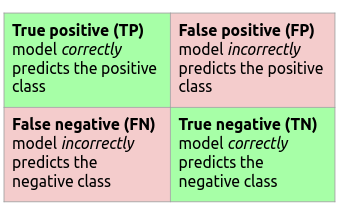
\includegraphics[scale=0.5]{chapters/images/conf_mtx.png}
    \caption{A 2x2 confusion matrix. Source: \cite{olakka}}
    \label{fig:confusion_matrix}
\end{figure}

Accuracy (ACC) of the model is calculated as the number of all correct predictions divided by the total number of the dataset. The best accuracy is 1.0, whereas the worst is 0.0. Mathematically, 

\begin{equation}
    ACC = \frac{TP+TN}{TP+TN+FP+FN} = \frac{TP+TN}{P+N}
    \label{eq:accuracy}
\end{equation}


\subsection{Deployment}
Deployment comes next when the model has been assessed and proven to have satisfactory performance. We often specify a minimal accuracy threshold value, and if the observed accuracy falls below the threshold, the model is discarded otherwise accepted. The constantly changing nature of data necessitates periodic model evaluation and performance verification.  